\documentclass{extbook}
\usepackage[papersize={8.5in,11in},top=1in,bottom=1in]{geometry}
\RequirePackage{fix-cm}
\usepackage[T1]{fontenc}
\usepackage{lmodern}
\usepackage{fullpage}
\usepackage{titlesec}
\usepackage{parskip}
\usepackage{float}
\usepackage{url}
\usepackage[pdfauthor={Arland Barrera}, 
pdftitle={Laboratorio V Base de Datos II}, 
pdfsubject={https://github.com/ArlandBarrera/DBII{\textunderscore}Laboratorio{\textunderscore}5}]
{hyperref}
\usepackage{graphicx}
\usepackage{tcolorbox}
\usepackage{tabularx}
\usepackage{xcolor}
\usepackage{titlesec}
\usepackage{amsmath}
\usepackage{tcolorbox}
\usepackage{tabularx}

\renewcommand{\contentsname}{Contenido}
\renewcommand{\figurename}{Figura}
%\renewcommand{\listtablename}{Lista de tablas}
\renewcommand{\listfigurename}{Lista de figuras}
\usepackage[fontsize=13.5pt]{fontsize}
\setlength{\parindent}{0pt}

\titleformat{\chapter}[display]
  {\bfseries\huge} % Estilo del título
  {\hfill\Large} % Alineación a la derecha
  {3ex} % Espaciado entre el número del capítulo y el título
  {\vspace{-5cm}\titlerule\vspace{1.5ex}\hfill} % Regla arriba y alineación del título a la derecha
  [\vspace{1ex}\titlerule] % Regla debajo del título


  \makeatletter
  \patchcmd{\chapter}
    {\if@openright\cleardoublepage\else\clearpage\fi}
    {\clearpage}
    {}{}
  \makeatother

  \definecolor{codegreen}{rgb}{0,0.6,0}
  \definecolor{codegray}{rgb}{0.5,0.5,0.5}
  \definecolor{codepurple}{rgb}{0.58,0,0.82}
  \definecolor{backcolour}{rgb}{0.95,0.95,0.92}

\begin{document}
\begin{titlepage}
  \begin{center}
      {\huge \textbf{Universidad Tecnológica de Panamá}}\\
      \vspace{3mm}
      {\Large \textbf{Centro Regional De Veraguas}}

      \begin{figure}[H]
          \centering
          
\includegraphics[scale = 0.07]{Imagenes/UTP/utp.png}
          
\includegraphics[scale = 0.58]{Imagenes/UTP/fisc.png}
      \end{figure}
      {\Large \textbf{Facultad de Ingeniería de Sistemas Computacionales}}\\
      \vspace{5mm}
      
      {\Large \textbf{Curso: Base de Datos II}}\medskip
      
      {\Large \textbf{Profesor: Carlos Herrera}}

      \rule{\linewidth}{0.75mm}\\
          {\Large \textsc{Laboratorio 5}} 
      \rule{\linewidth}{0.75mm}\medskip

      {\Large \textbf{Estudiante}}\\
      \vspace{5mm}
      {\Large \textbf{Arland Barrera}}
      \vfill
      {\Huge \textbf{2024}}

  \end{center}
\end{titlepage}
\tableofcontents
\listoffigures
%\listoftables para lista de tablas
\chapter{Desarrollo}
\section{Parte 1: Creación de la Base de Datos y Colecciones}
Crear la base de datos \emph{universidad} en \textit{Mongo Shell}:

\begin{figure}[H]
  \centering
  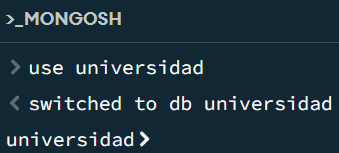
\includegraphics{Imagenes/parte1/1.1.png}
  \caption{Creación de la base de datos universidad}
\end{figure}

Crear la colección \emph{`estudiantes'}:

\begin{figure}[H]
  \centering
  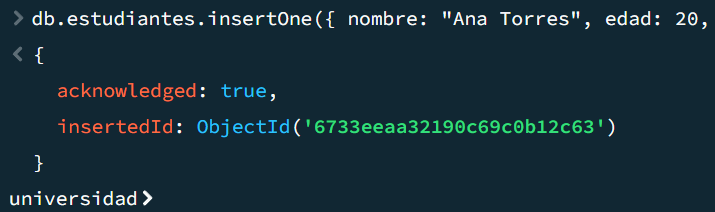
\includegraphics[scale = 0.8]{Imagenes/parte1/1.2.png}
  \caption{Creación de la colección estudiantes}
\end{figure}

Crear la colección \emph{`cursos'}:

\begin{figure}[H]
  \centering
  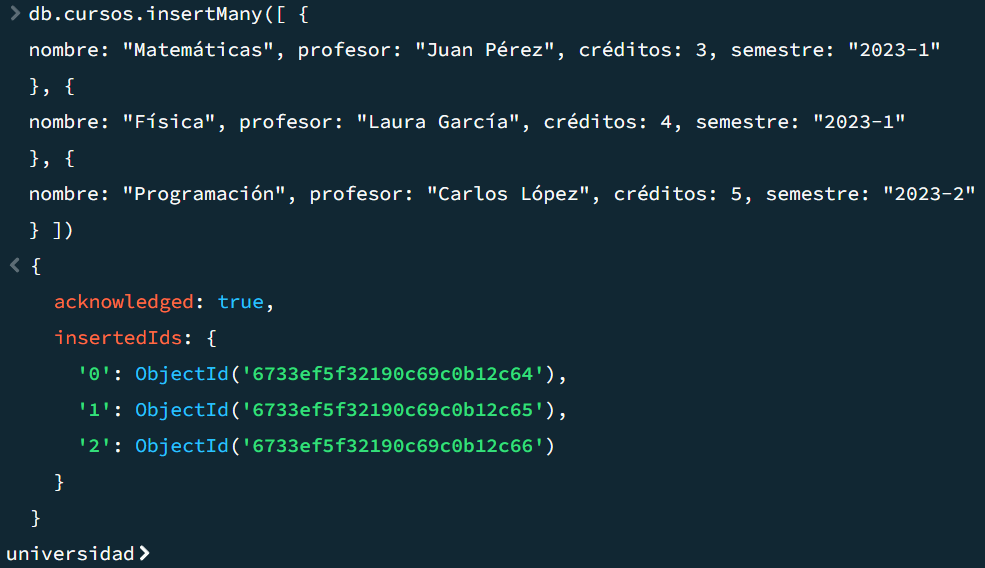
\includegraphics[scale = 0.5]{Imagenes/parte1/1.3.png}
  \caption{Creación de la colección cursos}
\end{figure}
\section{Parte 2: Insertar Documentos en la Colección `estudiantes'}
Agregar más estudiantes a la colección \emph{`estudiantes'}:

\begin{figure}[H]
  \centering
  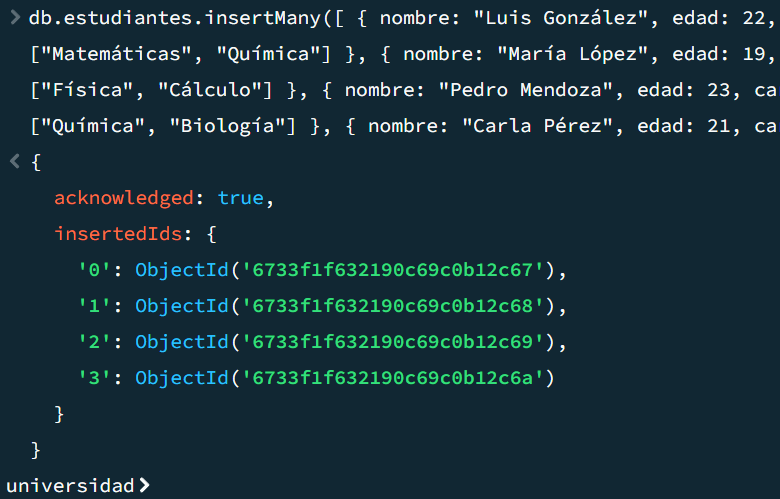
\includegraphics[scale = 0.6]{Imagenes/parte2/2.1.png}
  \caption{Agregar documentos a la colección estudiantes}
\end{figure}
\section{Parte 3: Consultas Básicas con Operadores Relacionales}
\textbf{Consulta básica}: Encontrar todos los estudiantes de la carrera de \textit{`Ingeniería'}:

\begin{figure}[H]
  \centering
  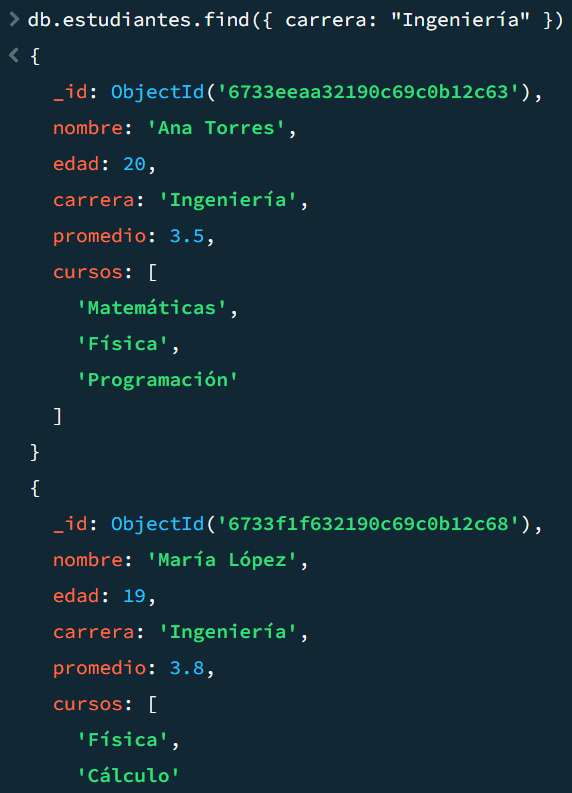
\includegraphics[scale = 0.8]{Imagenes/parte3/3.1.png}
  \caption{Consulta básica}
\end{figure}

\textbf{Operador de comparación \emph{\$gt}}: Obtener estudiantes con un \textit{promedio superior a 3.5}:

\begin{figure}[H]
  \centering
  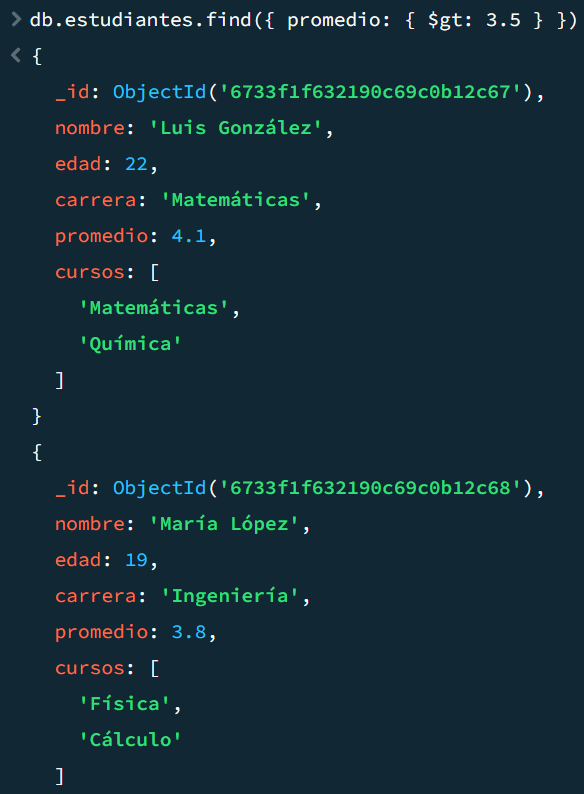
\includegraphics[scale = 0.8]{Imagenes/parte3/3.2.png}
  \caption{Consulta gt}
\end{figure}

\textbf{Operador de comparación \emph{\$lt}}: Buscar estudiantes \textit{menores de 21 años}:

\begin{figure}[H]
  \centering
  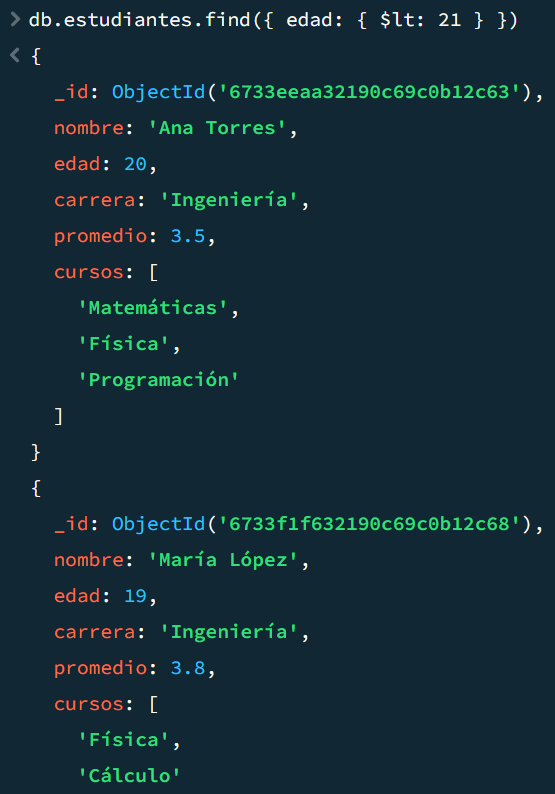
\includegraphics[scale = 0.8]{Imagenes/parte3/3.3.png}
  \caption{Consulta lt}
\end{figure}

\textbf{Operador \emph{\$in}}: Encontrar estudiantes que están \textit{inscritos en el curso de `Matemáticas' o `Física'}:

\begin{figure}[H]
  \centering
  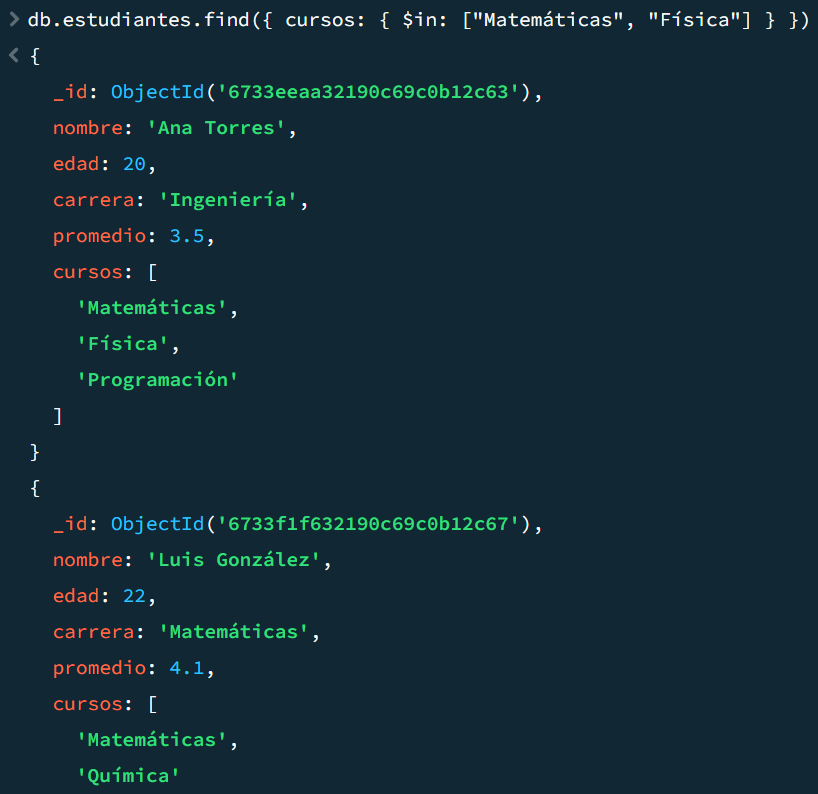
\includegraphics[scale = 0.8]{Imagenes/parte3/3.4.png}
  \caption{Consulta in}
\end{figure}

\textbf{Operador \emph{\$and}}: Obtener estudiantes de la \textit{carrera de `Ingeniería' con un promedio mayor a 3.5}:

\begin{figure}[H]
  \centering
  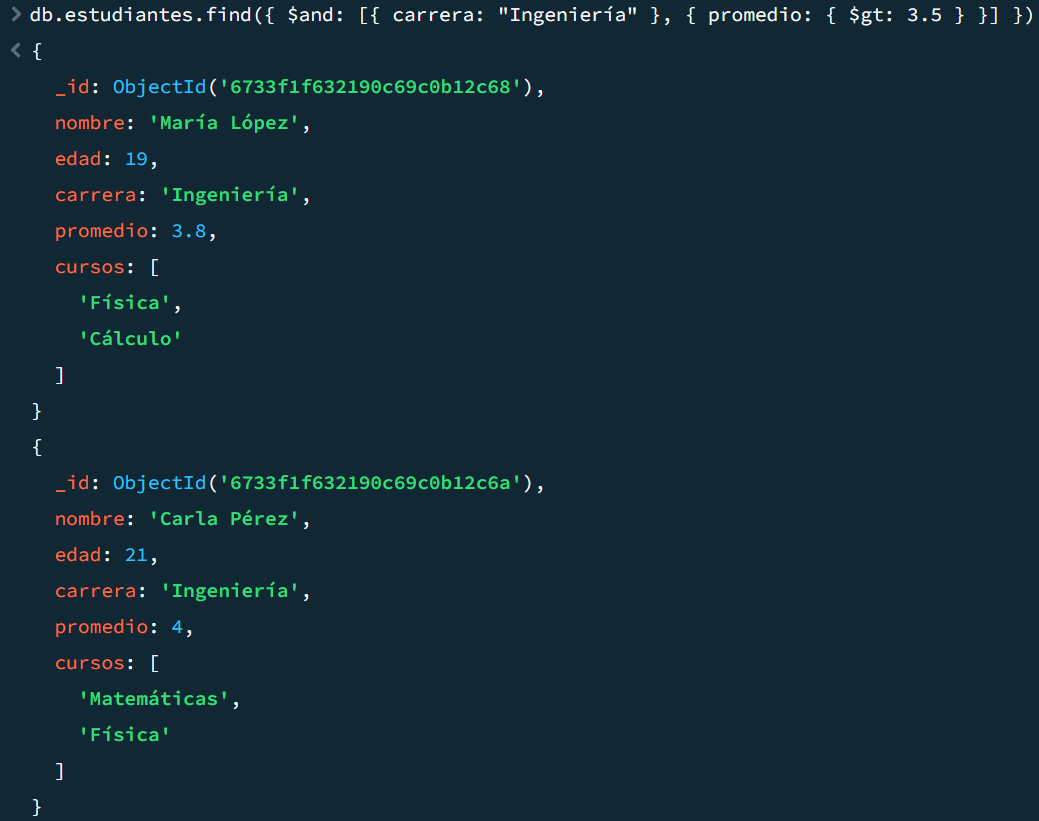
\includegraphics[scale = 0.6]{Imagenes/parte3/3.5.png}
  \caption{Consulta and}
\end{figure}

\textbf{Operador \emph{\$or}}: Obtener estudiantes cuyo \textit{promedio sea mayor a 4.0 o que estén en el curso de `Biología'}:

\begin{figure}[H]
  \centering
  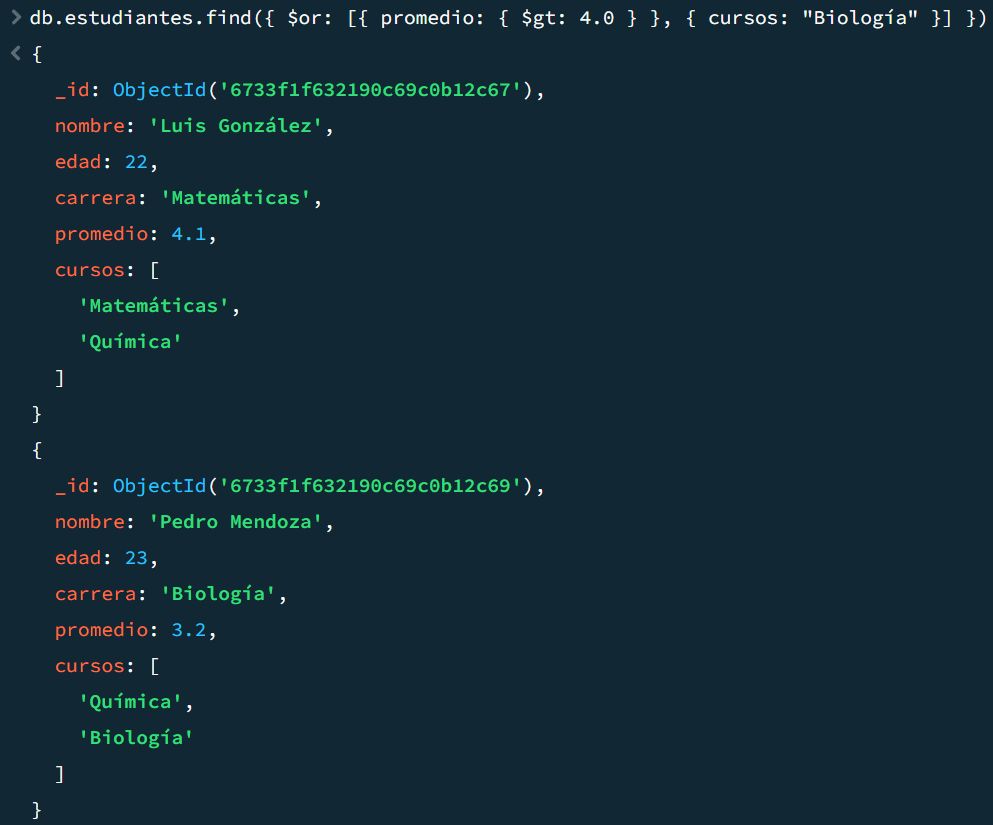
\includegraphics[scale = 0.6]{Imagenes/parte3/3.6.png}
  \caption{Consulta or}
\end{figure}

\textbf{Consulta de proyección}: Mostrar solo los \textit{nombres y promedios} de los estudiantes:

\begin{figure}[H]
  \centering
  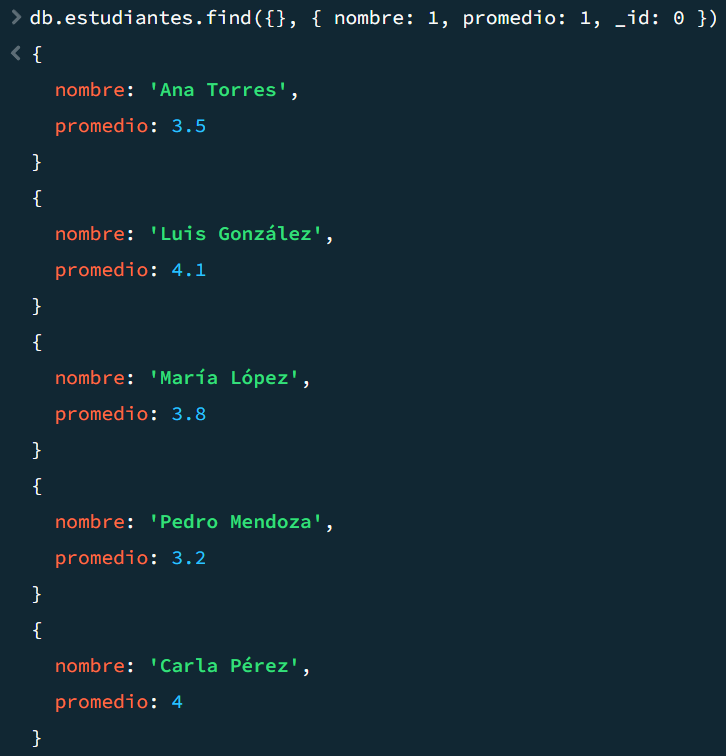
\includegraphics[scale = 0.8]{Imagenes/parte3/3.7.png}
  \caption{Consulta de proyección}
\end{figure}
\end{document}